%!TEX root = ../Main.tex

\chapter{implementation}

\section{Overview}
To give an overview of the software for the system, a class diagram has been made. This can be seen on \cref{fig:ClassDiagram}.
The class diagram have been developed based on the former domain problem analysis such as use cases. When a class diagram has been made that complies with the aforementioned use cases, it was used as a guideline for developing the system. Some changes have been made throughout the development when smarter options became apparent. \cref{fig:ClassDiagram} shows the latest class diagram for ROGSAnne.

\begin{figure}[H]
	\centering
	{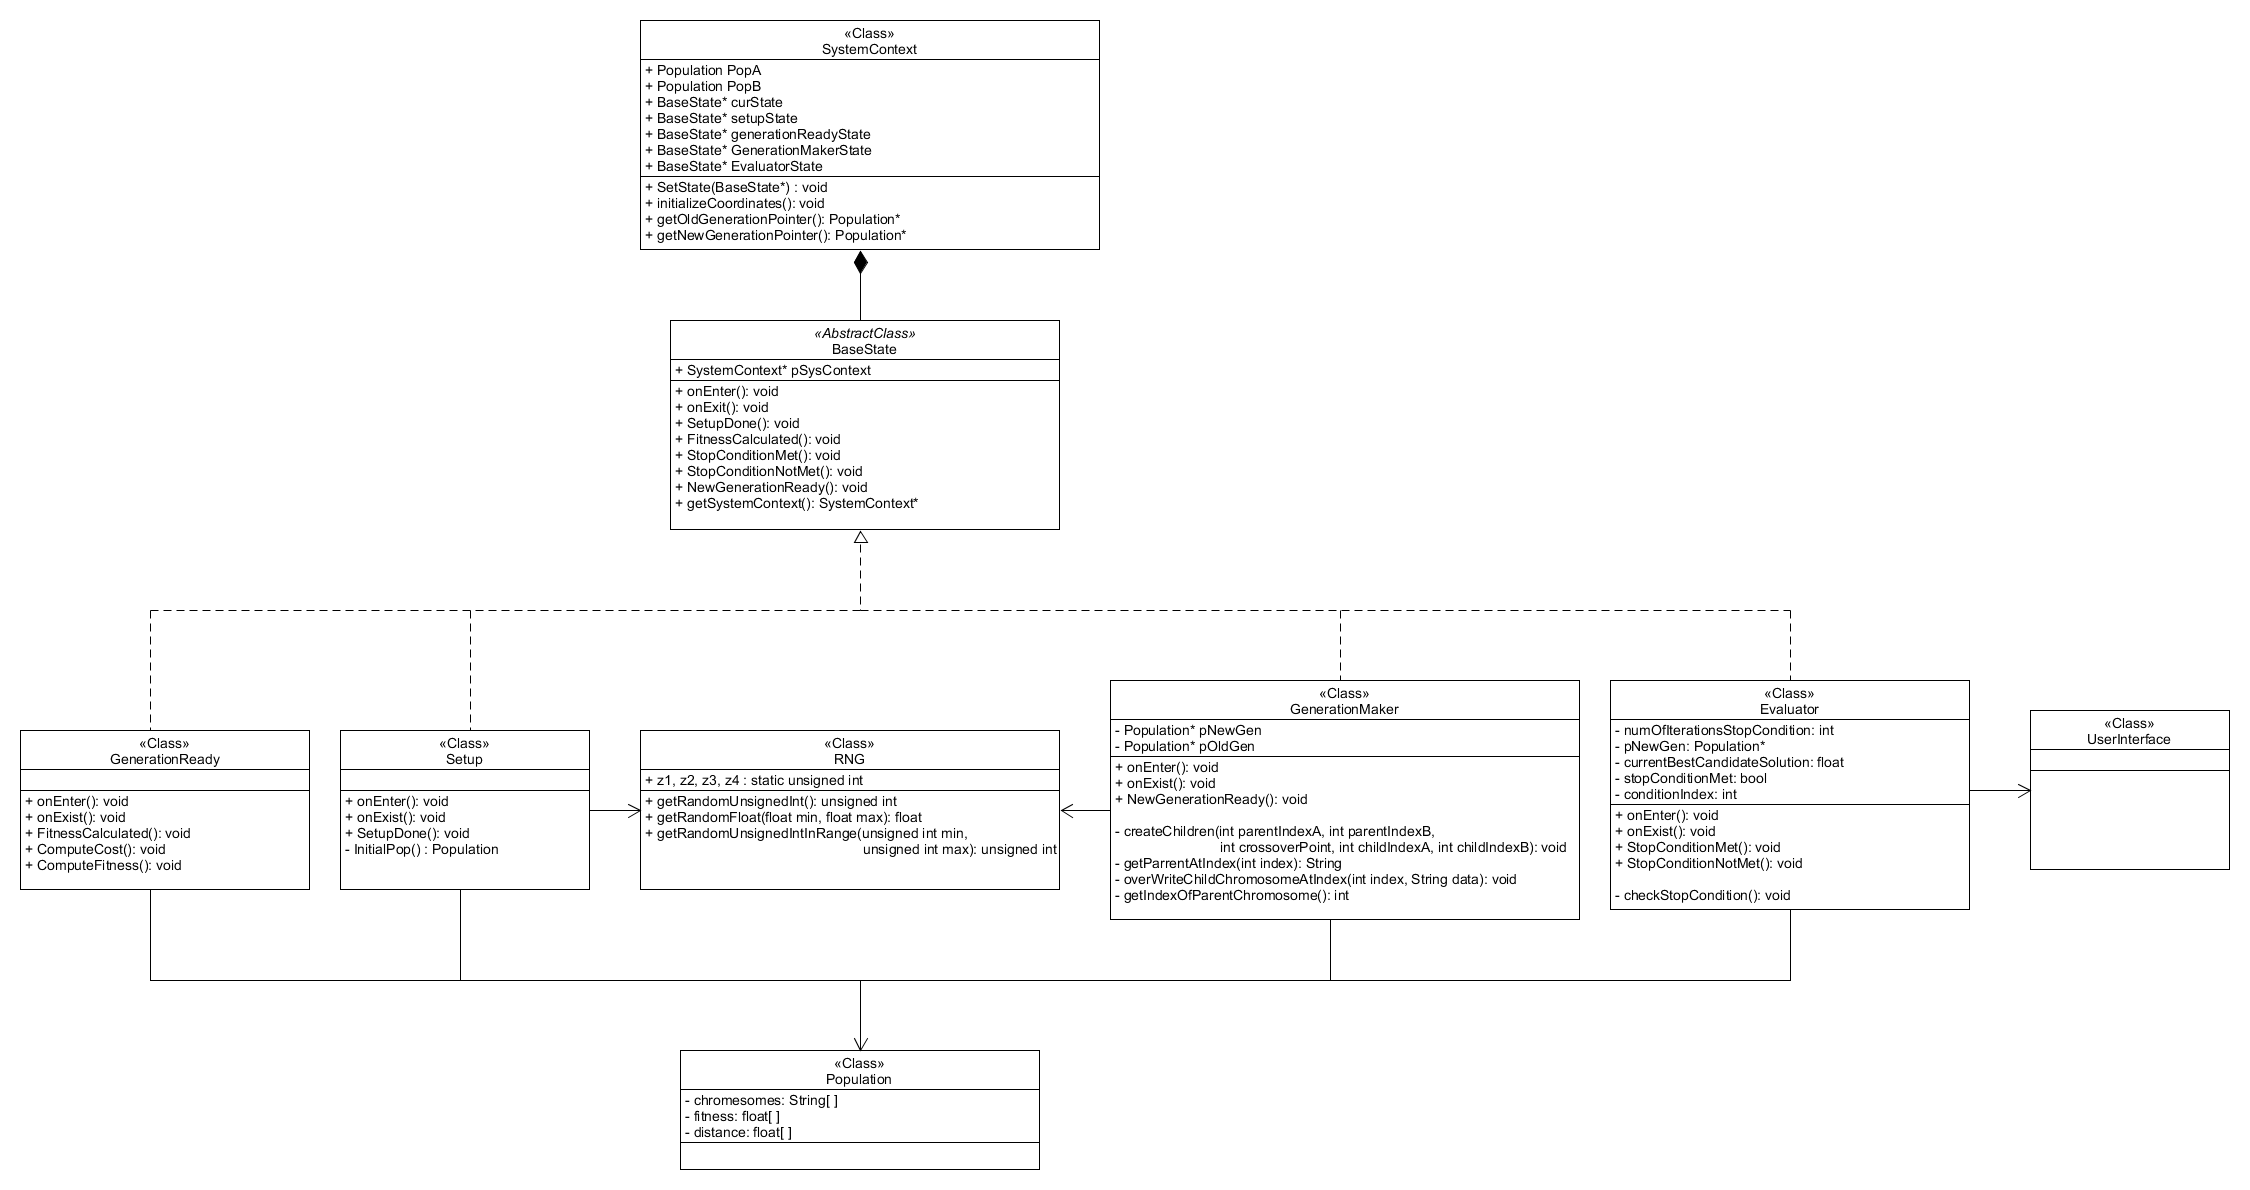
\includegraphics[width=\textwidth]{Images/ClassDiagram.PNG}}\\[0.5cm]
	\caption{Class diagram for the developed system.}
	\label{fig:ClassDiagram}
\end{figure}

As mentioned in the Design chapter a State Machine pattern has been chosen as a good fit for this system and a \textbf{SystemContext} class has been made to handle the holding and switching of states. The abstract class \textbf{Statebase} has virtual methods of each event needed for switching between states. Because StateBase is abstract each state class that inherits from the class needs to implement the corresponding method for changing state. I.e GenerationReady needs to implement FitnessCalculated() otherwise a default version will be called and an exception is called.

The four states functionality is described under the design chapter and can be summed up to:

\begin{itemize}
	\item \textbf{Setup}: Create initial population
	\item \textbf{GenerationReady}: Calculate distance and fitness of population
	\item \textbf{Evaluator}: Checks if there's been generated a better candidate solution, if not increment a counter. If this counter reaches a certain value, our stop condition is met and the program ends.
	\item \textbf{GenerationMaker}: Generate new population by taking the best of the population and use them as parents.
\end{itemize}


\subsection{Timer}
One of the requirements for this assignment was to implement and test a part of the systems functionality on the ZYBO-board. So, different functionalities of the system were timed to examine what functionality of the system is most time consuming. To time the different functionalities a TimerClass was implemented. The class diagram for the TimerClass can be seen on \cref{fig:TimerClass_CD}. The library \textbf{XScuTimer.h} were used. 
\begin{figure}[H]
	\centering
	{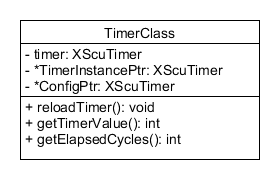
\includegraphics[width=\textwidth/2]{Images/TimerClass_CD.PNG}}\\[0.5cm]
	\caption{Class diagram for the TimerClass.}
	\label{fig:TimerClass_CD}
\end{figure}

The idea was to measure the most time consuming functionality in the system and hardware accelerate that functionality on the ZYBO-board and test the improvement. Three functionalities were time; the calculation of distance for each population, the calculation of fitness for each population and the generation of a new generation. Each of the functionalities were timed five times and the were mean calculated. On \cref{fig:timing_barGraph} a bar-graph of the timing results are presented. 

\begin{figure}[H]
	\centering
	{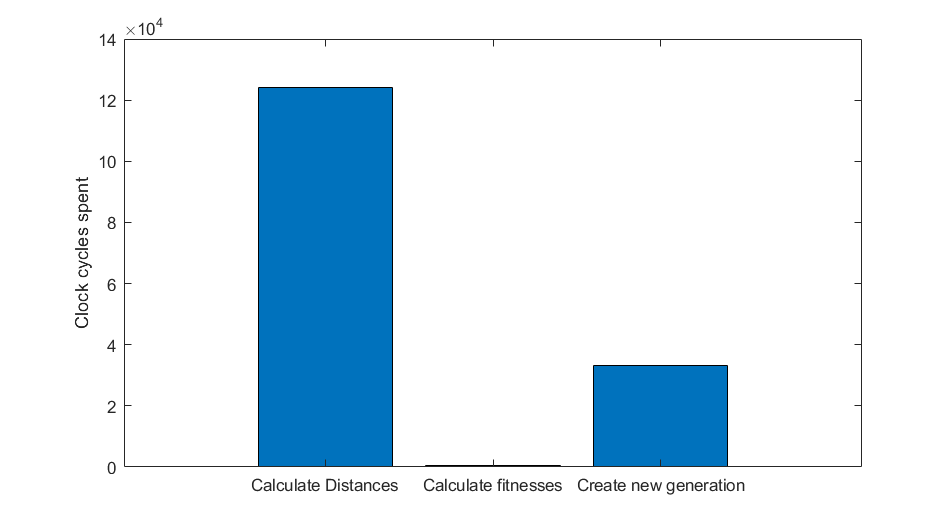
\includegraphics[width=\textwidth]{Images/timing_barGraph.png}}\\[0.5cm]
	\caption{Timing of functionalities bar-graph}
	\label{fig:timing_barGraph}
\end{figure}

Its clear that the calculation of distances is the most time consuming functionality. So, this functionality will be hardware accelerated on the ZYBO-board.


\section{Test of system}
10 predetermined coordinates has been hardcoded into the program. The setup class makes an initial population each with these 10 coordinates in a random order. The population is evaluated and a new population is made based on the best performing of the population. Whenever a new better solution(population) is found, this is saved as the best so far. If no better solution is found after 19 iteration, the program stops and the best solution has been found. An example of this can be seen below on \cref{fig:algo_test_sw}.

\begin{figure}[H]
	\centering
	{\includegraphics[width=\textwidth/2]{Images/algo_test_sw.png}}\\[0.5cm]
	\caption{Test of genetic algorithm}
	\label{fig:algo_test_sw}
\end{figure}

\section{SystemC}
In order to improve system speed, a hardware acceleration of the module computing the distances is made. This is done using the tool Vivado HLS, which is a tool used for high level synthesis. This was done by implementing the module in SystemC, creating a testbench to test the module, and then synthesizing the module. \Cref{list:DistCalcH} shows the header file for the SystemC module, specifying the interfaces to and from the module. Apart from the standard clock- and reset-signals it has the following:

\begin{description}
	\item[x and y] Inputs in form of two fifos, from which the x- and y-coordinates of the points are read in order of appearance in the route.
	\item[outputDist] The output from the IP where the calculated distance will be read from.
	\item[numberOfPoints] An indicator of how many entries in the FIFO-buffers that carry actual information. This is done because of implementation reasons, as it was necessary to always pass a set number of points in order to know about the timing of the module. A maximum of 10 points can be passed. If fewer are to be calculated, the data in the last entries are irrelevant.	
	\item [ready] A boolean signal indicating whether data has been written to the FIFOs.
	\item [busy] A boolean signal indicating whether the module is still performing calculations, or whether a result is ready. When false, a result is ready.
\end{description}
Furthermore, the constructor just instantiates a clocked thread, running the method DistCalcThread, as seen in \cref{list:DistCalcCPP}. The thread waits until it reads a high ready-signal, indicating that data is ready in the FIFOs. It then indicates that it's busy, and starts to calculate the distance given the provided points and the number of points to calculate for. Once calculation is done, the result is written to the output. and the busy-signal is set low, indicating that a result is ready. The thread will then just wait until its ready-signal is high again.

Line 32 shows a "directive" used in the synthesis of the module in order to improve performance. This particular directive indicates that the for-loop should be "unrolled" meaning, that the loop is being split in 3 separate loops, that can be executed in parallel. The number 3 comes from a trial-and-error test, in which it was found that an unroll factor of 3 was the optimal choice in regards to speed (see section [REF SECTION PARETO-THINGY]).

\captionsetup[lstlisting]{font={small,tt}}
\lstinputlisting[language=c++, caption = header file for Distance Calculator module., label = list:DistCalcH]{../Bilag/CodeCopy/DistCalc.h}

\captionsetup[lstlisting]{font={small,tt}}
\lstinputlisting[language=c++, caption = source code for Distance Calculator module., label = list:DistCalcCPP]{../Bilag/CodeCopy/DistCalc.cpp}

\Cref{list:DistCalcDriverH} and \cref{list:DistCalcDriverCPP} shows the driver used to test the module. In it, a series of points is written to the DUT("Device under test"), and the resulting output is compared to and expected value, calculated in MATLAB.

\Cref{list:DistCalcTBCPP} shows the testbench set up for testing the module. In it, a set of signals is created, and the an instance of the driver and the DUT is created, after which these are connected to the signals. Then, simulation runs for 200ns, and based on the return value from the driver, it is indicated whether the test passed or failed. Furthermore, the state of the signals throughout the simulation is written to a tracefile.

\captionsetup[lstlisting]{font={small,tt}}
\lstinputlisting[language=c++, caption = source code for Distance Calculator Driver., label = list:DistCalcDriverH]{../Bilag/CodeCopy/DistCalcDriver.h}

\captionsetup[lstlisting]{font={small,tt}}
\lstinputlisting[language=c++, caption = source code for Distance Calculator Driver., label = list:DistCalcDriverCPP]{../Bilag/CodeCopy/DistCalcDriver.cpp}

\captionsetup[lstlisting]{font={small,tt}}
\lstinputlisting[language=c++, caption = source code for Distance Calculator test bench., label = list:DistCalcTBCPP]{../Bilag/CodeCopy/tb_DistCalc.cpp}

\subsection{Design space exploration}
During implementation of the module, it was found that using the "unroll"-directive during synthesis to unroll the for-loop in the module thread increased performance in terms of latency/calculation time. Initially, the directive was applied with no unroll factor. This increased in a very high performance, but with an estimated clock higher than the target clock (8.35 vs. 8.00), which is not a viable design. Thus, the directive was tried with different unroll factors. The module was synthesized using different unroll factors, and the estimated clock and latency was noted. The results can be seen in \cref{fig:design_space_diagram}. It is seen that while a full unroll results in the best latency, the resulting estimated clock is above the max tolerated clock. The lowest latency that also results in a tolerated clock is obtained, when using an unroll factor of 3, which is why this is chosen in the final implementation of the module.
\begin{figure}[H]
	\centering
	{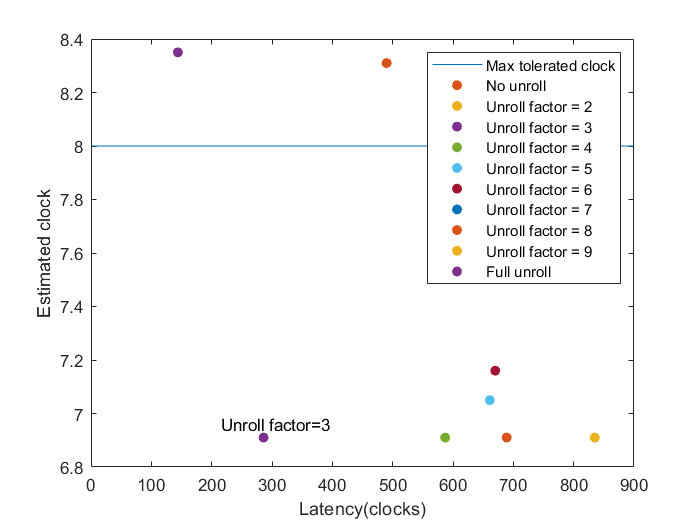
\includegraphics[width=\textwidth/2]{Images/paerto_latency_clock.PNG}}\\[0.5cm]
	\caption{Design space diagram, comparing estimated clock and latency.}
	\label{fig:design_space_diagram}
\end{figure}